%        File: HW2.tex
%     Created: Tue Feb 22 09:00 AM 2011 C
% Last Change: Tue Feb 22 09:00 AM 2011 C
%
\documentclass[letterpaper]{article}
\usepackage{amsmath,amsfonts}
\usepackage[margin=1.25in]{geometry}
\usepackage[]{graphicx}
\usepackage{listings}
\usepackage{color}
\usepackage{textcomp}
\definecolor{listinggray}{gray}{0.9}
\definecolor{lbcolor}{rgb}{0.9,0.9,0.9}
\lstset{
	backgroundcolor=\color{lbcolor},
	tabsize=4,
	rulecolor=,
% 	language=Python,
        basicstyle=\scriptsize,
        upquote=true,
        aboveskip={1.5\baselineskip},
        columns=fixed,
        showstringspaces=false,
        extendedchars=true,
        breaklines=true,
        prebreak = \raisebox{0ex}[0ex][0ex]{\ensuremath{\hookleftarrow}},
        frame=single,
        showtabs=false,
        showspaces=false,
        showstringspaces=false,
        identifierstyle=\ttfamily,
        keywordstyle=\color[rgb]{0,0,1},
        commentstyle=\color[rgb]{0.133,0.545,0.133},
        stringstyle=\color[rgb]{0.627,0.126,0.941},
}

\begin{document}
\section*{Problem 3}
The first step in designing the grid was to find an appropriate integration
range. The integral of interest is
\[
Z=\int_{\mathbb{R}^2}e^{-\beta U(x,y)}dxdy\,.
\]
The exponent will blow up away from the origin, so we need to find a range such
that the integrand becomes essentially zero. The smallest $\beta$ that we will
be plotting is $\beta=0.01$. If we do a contour plot of the integrand for this
smallest $\beta$ we can find a safe range to perform our numerical integration
for all $\beta$.
\begin{figure}[h]
\begin{center}
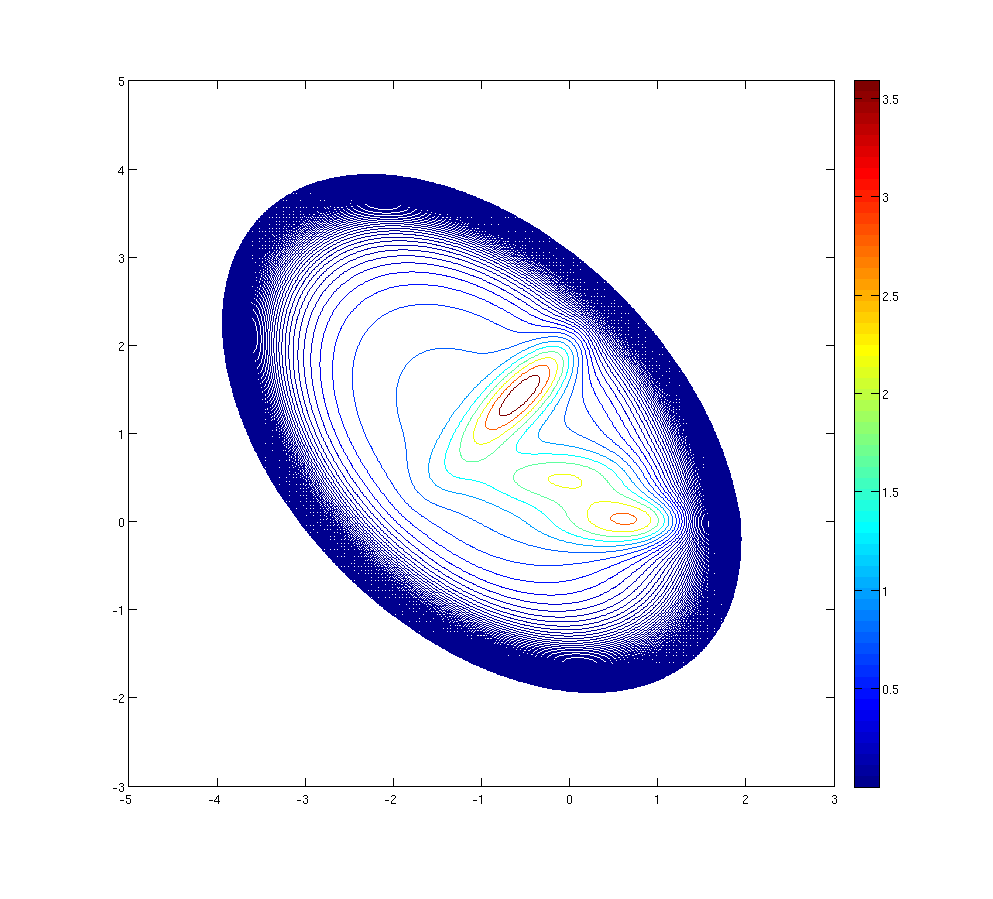
\includegraphics[width=5in,keepaspectratio]{Integrand.png}
\end{center}
\caption{Contour plot of $\exp(-\beta U(x,y))$ for $\beta=0.01$}
\label{fig:integrand}
\end{figure}
Figure \ref{fig:integrand} indicates that a safe domain of integration would be
$-5\le x\le 3$ and $-3\le y\le 5$.

The next task is to choose an appropriate numerical quadrature method. Ideally,
we would like to concentrate our efforts on the part of the function that is
changing more rapidly, but I decided to go with a uniform refinement Riemann
integration for its simplicity and predictable convergence properties. I
discovered that the interesting range of $\beta$ was $0.01\le\beta\le 1$.
Running a couple of resolution tests at the extremes: for $\beta=0.01$ and a
$50\times50$ grid $\frac{-1}{\beta}\log(Z)=-236.0067$. At double the resolution,
I got $-238.0375$, so the first two digits are accurate as desired. For
$\beta=1$ the results at $50\times50$ and $100\times100$ were $-145.8771$ and
$-146.1914$, respectively. So we can conclude that a $50\times50$ grid is
accurate enough.

We encounter another numerical difficulty when attempting to evaluate our
integral. The Muller potential has a minimum value of approximately $-145$, so
when we evaluate $e^{-\beta(-145)}=e^{145\beta}$, for moderate $\beta$, our
integrand blows up and approaches the machine overflow, losing a lot of accuracy
in the process. We can perform a little numerical trick as follows
\begin{align*}
F&=\frac{-1}{\beta}\log\left(\int e^{-\beta U(x,y)}dxdy\right)\\
&=\frac{-1}{\beta}\log\left(\int e^{-\beta U_{min}}e^{-\beta
(U(x,y)-U_{min})}\right)\\
&=\frac{-1}{\beta}\log\left(e^{-\beta U_{min}}\int e^{-\beta
(U(x,y)-U_{min})}\right)\\
&=U_{min}+\frac{-1}{\beta}\log\left(\int e^{-\beta
(U(x,y)-U_{min})}\right)\,,
\end{align*}
where $U_{min}$ is some offset on the order of the minimum potential which makes
the integral easier to evaluate numerically. For our purposes, we use
$U_{min}=-145$, which appears to produce good results for a variety of $\beta$.

The calculation time is, of course going to depend heavily on the chosen mesh
resolution and number of plot points. With our $50\times50$ grid, each
integration takes an average of $0.05$ seconds. With 50 plot points, this comes
out to a total runtime of approximately $2.5$ seconds.

Figure \ref{fig:freeenergy} plots the free energy $F=-\beta^{-1}\log(Z)$ as a
function of $\beta$.
\begin{figure}[h]
\begin{center}
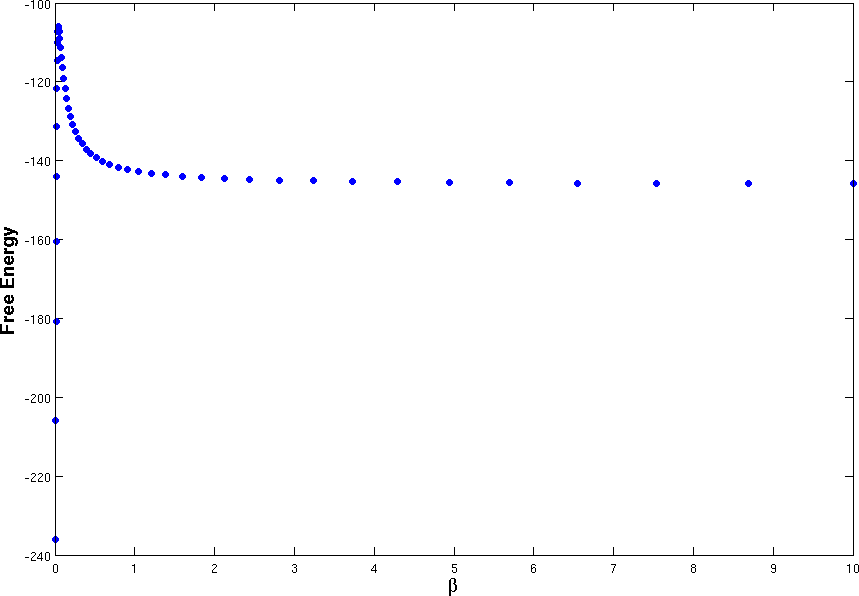
\includegraphics[width=5in,keepaspectratio]{FreeEnergy.png}
\end{center}
\caption{Free energy versus $\beta$}
\label{fig:freeenergy}
\end{figure}

\newpage 
\clearpage
\lstinputlisting[language=Matlab,title={PlotMuller.m}]{PlotMuller.m}
\end{document}
